\documentclass[a4paper,11pt,exos]{nsi} % COMPILE WITH DRAFT
\usepackage{pifont}
\usepackage{fontawesome5}

\begin{document}
\classe{\premiere spé}
\titre{Corrigé - Premier degré}
\maketitle

\subsection*{Premier degré}
\exo{}
\begin{enumerate}
    \item 	\setlength{\columnseprule}{0pt}
    \begin{multicols}{2}
        \begin{enumerate}[label=\textbullet]
            \item 	\begin{tabbing}
                $\qquad$ \= $2x+8=0$\\
                $\Longleftrightarrow$   \>  $2x=-8$\\
                $\Longleftrightarrow$   \>  $\dfrac{2x}{2}=-\dfrac{8}{2}$\\
                $\Longleftrightarrow$   \>  $x=-4$
            \end{tabbing}
            $\mathcal{S}=\left\{-4\right\}$
            \item 	\begin{tabbing}
                $\qquad$ \= $-3x+18=0$\\
                $\Longleftrightarrow$   \>  $-3x=-18$\\
                $\Longleftrightarrow$   \>  $\dfrac{-3x}{-3}=\dfrac{-18}{-3}$\\
                $\Longleftrightarrow$   \>  $x=6$
            \end{tabbing}
            $\mathcal{S}=\left\{6\right\}$
            \vfill\null
            \columnbreak

            \item 	\begin{tabbing}
                $\qquad$ \= $-\dfrac{12}{7}x+\dfrac{4}{21}=0$\\[.5em]
                $\Longleftrightarrow$   \>  $-\dfrac{12}{7}x=-\dfrac{4}{21}$\\[.5em]
                $\Longleftrightarrow$   \>  $-\dfrac{7}{12}\times\left(-\dfrac{12}{7}\right)x=-\dfrac{7}{12}\times\left(-\dfrac{4}{21}\right)$\\[.5em]
                $\Longleftrightarrow$   \>  $x=\dfrac{7\times4}{12\times21}$\\[.5em]
                $\Longleftrightarrow$   \>  $x=\dfrac{1}{9}$
            \end{tabbing}
            $\mathcal{S}=\left\{\dfrac{1}{9}\right\}$
            \item 	\begin{tabbing}
                $\qquad$    \=   $\sqrt{2}x-1=0$\\
                $\Longleftrightarrow$   \>  $\sqrt{2}x=1$\\
                $\Longleftrightarrow$   \>  $x=\dfrac{1}{\sqrt{2}}$\\
                $\Longleftrightarrow$   \>  $x=\dfrac{\sqrt{2}}{2}$
            \end{tabbing}
            $\mathcal{S}=\left\{\dfrac{\sqrt{2}}{2}\right\}$
        \end{enumerate}
    \end{multicols}
    \item	
    \begin{tabbing}
        $\qquad$    \=  $ax+b=0$\\
        $\Longleftrightarrow$   \>  $ax=-b$\\
        $\Longleftrightarrow$   \>  $\dfrac{ax}{a}=\dfrac{-b}{a}$\\
        $\Longleftrightarrow$   \>  $x=-\dfrac{b}{a}$
    \end{tabbing}
    $\mathcal{S}=\left\{-\dfrac{b}{a}\right\}$
\end{enumerate}


\exo{}
\textbf{\textsc{Partie A}}
	\begin{enumerate}
		\item 	$\pc{A}{1}{6}\ ; \quad \pc{B}{6}{4}$
		\item 	\begin{tabbing}
            $m$ \=  $=\dfrac{y_B-y_A}{x_B-x_A}$\\[.5em]
                \>  $=\dfrac{4-6}{6-1}$\\[.5em]
                \>  $=-\dfrac{2}{5}$
        \end{tabbing}
		\item 	On peut lire $p\approx 6,5$.
		\item 	La droite $(AB)$ a pour équation réduite $\quad y=-\dfrac{2}{5}x+p \quad$ avec $p$ un réel à déterminer.\\
		Le point $A$ appartient à la droite $(AB)$ donc ses coordonnées vérifient l'équation précédente.
        \begin{tabbing}
            $\qquad$    \=  $y_A=-\dfrac{2}{5}x_A+p$\\[.5em]
            $\Longleftrightarrow$   \>  $6=-\dfrac{2}{5}\times 1+p$\\[.5em]
            $\Longleftrightarrow$   \>  $6+\dfrac{2}{5}=p$\\[.5em]
            $\Longleftrightarrow$   \>  $\dfrac{30}{5}+\dfrac{2}{5}=p$\\[.5em]
            $\Longleftrightarrow$   \>  $p=\dfrac{32}{5}$
        \end{tabbing}
        La droite $(AB)$ a donc pour équation réduite $\quad y=-\dfrac{2}{5}x+\dfrac{32}{5}$.
	\end{enumerate}



	\textbf{\textsc{Partie B}}
	On considère les 2 fonctions affines $f$ et $g$ définies sur $\R$ par : $\ f(x)=\dfrac{1}{3}x-2\ $ et $\ g(x)=-3x+6$.
	
    \begin{multicols}{2}
        \begin{enumerate}
            \item 	\begin{tabbing}
                $f(0)$ \=   $=\dfrac{1}{3}\times 0-2$\\[.5em]
                    \>  $=-2$
            \end{tabbing}
            \item 	\begin{tabbing}
                $\qquad$    \=  $f(x)=0$\\
                $\Longleftrightarrow$   \>  $\dfrac{1}{3}x-2=0$\\[.5em]
                $\Longleftrightarrow$   \>  $\dfrac{1}{3}x=2$\\[.5em]
                $\Longleftrightarrow$   \>  $3\times \dfrac{1}{3}x=3\times2$\\
                $\Longleftrightarrow$   \>  $x=6$
            \end{tabbing}
            $\mathcal{S}=\left\{6\right\}$
            \item 	$f$ est une fonction affine, $\courbe{f}$ est donc une droite.
            \item 	 $\courbe{f}$ est représentée en orange dans le repère.
            
            \item	\begin{tabbing}
                $g(0)$ \=   $=-3\times 0+6$\\[.5em]
                    \>  $=6$
            \end{tabbing}
            
            \begin{tabbing}
                $\qquad$    \=  $g(x)=0$\\
                $\Longleftrightarrow$   \>  $-3x+6=0$\\[.5em]
                $\Longleftrightarrow$   \>  $-3x=-6$\\[.5em]
                $\Longleftrightarrow$   \>  $\dfrac{-3x}{-3}x=\dfrac{-6}{-3}$\\
                $\Longleftrightarrow$   \>  $x=2$
            \end{tabbing}
            $\mathcal{S}=\left\{2\right\}$\\
            \vfill\null
            \columnbreak
            $\courbe{g}$ est représentée en rouge dans le repère.\\[.5em]
            \begin{tikzpicture}[scale = .7]
                \reperevl{-4}{-4}{8}{8}
                \clip (-4,-4) rectangle (8,8);
                \draw[thick,domain=-4:8,samples=2,variable=\x] plot ({\x},{6-2*(\x-1)/5});	
                \draw (1,6)node[above right]{A}\ball -- (6,4)node[above right]{B}\ball;	
                \draw[UGLiOrange,ultra thick,domain=-4:8,samples=2,variable=\x] plot ({\x},{\x/3-2});
                \draw[UGLiRed,ultra thick,domain=-4:8,samples=2,variable=\x] plot ({\x},{-3*\x+6});
                \draw [UGLiOrange] (-3,-3) node[below right] {$\courbe{f}$};
                \draw [UGLiRed] (3,-3) node[below right] {$\courbe{g}$};
            \end{tikzpicture}	
            \item 	\begin{tikzpicture}
                \tkzTabInit[lgt=3,espcl=2]
                {$x$ /.7 ,signe de $f(x)$ /.7}
                {$-\infty$, 6 ,$+\infty$ }
                \tkzTabLine{, -, z, +,}
            \end{tikzpicture}\\[.5em]
            \begin{tikzpicture}
                \tkzTabInit[lgt=3,espcl=2]
                {$x$ /.7 ,signe de $g(x)$ /.7}
                {$-\infty$, 2 ,$+\infty$ }
                \tkzTabLine{,+ , z,- ,}
            \end{tikzpicture}
        \end{enumerate}
    \end{multicols}
	



\subsection*{Fonctions affines}

\exo{}
%\begin{multicols}{3}
	\begin{enumerate}
		\item 	$f_1:x\mapsto-2x+1$\\
		$f_1$ est affine de taux d'accroissement $-2$ et d'ordonnée à l'origine $1$.
		\item 	$f_2:x\mapsto(2+x)(2x-1)$
		\begin{tabbing}
            $f_2(x)$ \= $=2\times 2x-2\times 1+x\times 2x-x\times 1$\\
            \>  $=4x-2+2x^2-x$\\
            \>  $=2x^2+3x-2$
        \end{tabbing}
        $f_2$ n'est pas une fonction affine.
		\item	$f_3:x\mapsto\dfrac{2x}{3}$\\
		$f_3(x)=\dfrac{2}{3}x+0$\\
        $f_3$ est affine de taux d'accroissement$\dfrac{2}{3}$ et d'ordonnée à l'origine $0$.
		\item	$f_4:x\mapsto\dfrac{1-2x}{3}$\\
		$f_4(x)=-\dfrac{2}{3}x+\dfrac{1}{3}$\\
        $f_4$ est affine de taux d'accroissement $-\dfrac{2}{3}$ et d'ordonnée à l'origine $\dfrac{1}{3}$.
		\item	$f_5:x\mapsto\dfrac{2}{3x}$\\
		$f_5$ n'est pas une fonction affine.
		\item	$f_6:x\mapsto x-(2x+1)$
		\begin{tabbing}
            $f_6(x)$\=  $x-2x-1$\\
            \>  $=-x-1$
        \end{tabbing}
        $f_6$ est affine de taux d'accroissement $-1$ et d'ordonnée à l'origine $-1$.
	\end{enumerate}
%\end{multicols}




\exo{}

\begin{multicols}{2}
	\begin{enumerate}
		\item 	$f_1$ est affine.\\
		$f_1(x)=\dfrac{3}{4}x-3$
        \def\xmin{-2}	\def\xmax{6}	\def\ymin{-5}	\def\ymax{2}
		\begin{center}
			\begin{tikzpicture}[scale = .58]
				\draw[fill=white](\xmin,\ymin) rectangle (\xmax,\ymax);
				\reperevl{\xmin}{\ymin}{\xmax}{\ymax}
				\clip (\xmin,\ymin) rectangle (\xmax,\ymax);
				\draw[ultra thick,color=UGLiRed,domain=\xmin:\xmax,samples=2,variable=\x] plot ({\x},{3/4*\x-3});
			\end{tikzpicture}
		\end{center}
	
		\item 	Cette droite ne représente pas une fonction.
        \def\xmin{-2}	\def\xmax{6}	\def\ymin{-5}	\def\ymax{2}
		\begin{center}
			\begin{tikzpicture}[scale = .58]
				\draw[fill=white](\xmin,\ymin) rectangle (\xmax,\ymax);
				\reperevl{\xmin}{\ymin}{\xmax}{\ymax}
				\clip (\xmin,\ymin) rectangle (\xmax,\ymax);
				\draw[ultra thick,color=UGLiDarkGreen] (3,-10) -- (3,10);
			\end{tikzpicture}
		\end{center}
\newpage
		\item 	$f_3$ est affine (elle est même linéaire).\\
        $f_3(x)=-x$
        \def\xmin{-2}	\def\xmax{6}	\def\ymin{-5}	\def\ymax{2}
		\begin{center}
			\begin{tikzpicture}[scale = .58]
				\draw[fill=white](\xmin,\ymin) rectangle (\xmax,\ymax);
				\reperevl{\xmin}{\ymin}{\xmax}{\ymax}
				\clip (\xmin,\ymin) rectangle (\xmax,\ymax);
				\draw[ultra thick,color=UGLiBlue,domain=\xmin:\xmax,samples=2,variable=\x] plot ({\x},{-\x});
			\end{tikzpicture}
		\end{center}
	
		\item 	$f_4$ est affine (elle est même constante).\\
        $f_4(x)=-2$
        \def\xmin{-2}	\def\xmax{6}	\def\ymin{-5}	\def\ymax{2}
		\begin{center}
			\begin{tikzpicture}[scale = .58]
				\draw[fill=white](\xmin,\ymin) rectangle (\xmax,\ymax);
				\reperevl{\xmin}{\ymin}{\xmax}{\ymax}
				\clip (\xmin,\ymin) rectangle (\xmax,\ymax);
				\draw[ultra thick,color=UGLiOrange,domain=\xmin:\xmax,samples=2,variable=\x] plot ({\x},{-2});
			\end{tikzpicture}
				\end{center}
	\end{enumerate}
\end{multicols}



\exo{}

\begin{multicols}{4}
	\begin{enumerate}
		\item 	$f:x\mapsto2x+1$
		\item 	$g:x\mapsto-3x+4$
		\item	$h:x\mapsto -2$
		\item	$k:x\mapsto -x-3$	
	\end{enumerate}
\end{multicols}
\def\xmin{-5}	\def\xmax{6}	\def\ymin{-5}	\def\ymax{6}
\begin{center}
	\begin{tikzpicture}[scale = 1]
		\draw[fill=white](\xmin,\ymin) rectangle (\xmax,\ymax);
		\reperevl{\xmin}{\ymin}{\xmax}{\ymax}
		\clip (\xmin,\ymin) rectangle (\xmax,\ymax);
        \draw[ultra thick,color=UGLiOrange,domain=\xmin:\xmax,samples=2,variable=\x] plot ({\x},{2*\x+1});
        \draw[UGLiOrange] (2.2,5) node[above right] {$(d_f)$};
        \draw[ultra thick,color=UGLiRed,domain=\xmin:\xmax,samples=2,variable=\x] plot ({\x},{-3*\x+4});
        \draw[UGLiRed] (-.5,5) node[above left] {$(d_g)$};
        \draw[ultra thick,color=UGLiDarkBlue,domain=\xmin:\xmax,samples=2,variable=\x] plot ({\x},{-2});
        \draw[UGLiDarkBlue] (-5,-1.5) node[right] {$(d_h)$};
        \draw[ultra thick,color=UGLiDarkGreen,domain=\xmin:\xmax,samples=2,variable=\x] plot ({\x},{-\x-3});
        \draw[UGLiDarkGreen] (-5,2) node[above right] {$(d_k)$};
	\end{tikzpicture}
\end{center}


\exo{}
%Donner le sens de variation des fonctions suivantes :
%\begin{multicols}{3}
	\begin{enumerate}
		\item 	$f:x\mapsto 3x-7$ \\
        $3>0$ donc $f$ est strictement croissante sur $\R$.
		\item 	$g:x\mapsto \dfrac{1}{2}x+9$\\
		$\dfrac{1}{2}>0$ donc $g$ est strictement croissante sur $\R$.
		\item	$h:x\mapsto -5x-2$\\
		$-5<0$ donc $h$ est strictement décroissante sur $\R$.	
	\end{enumerate}
%\end{multicols}


\exo{Vrai ou faux}
\begin{enumerate}
	\item 	%On considère une fonction affine $f$ croissante et telle que l’ordonnée à l’origine de sa représentation graphique est 3. On peut alors avoir $f(2) = 1$.	
	L'ordonnée à l'origine de $f$ est $3$ donc $\quad f(0)=3$.\\
	$f$ est croissante sur $\R$ donc $f(2)\geqslant f(0)$.\\
	On ne peut pas avoir $f(2) = 1$. L'affirmation est FAUSSE.
	\item 	%On considère une fonction affine $g$ décroissante et telle que l’ordonnée à l’origine de sa représentation graphique est 1. On peut alors avoir $g(2) = 0$.
	L'ordonnée à l'origine de $g$ est $1$ donc $\quad g(0)=1$.\\
	$g$ est décroissante sur $\R$ donc $g(2)\leqslant g(0)$.\\
	Il est possible de trouver une telle fonction $g$ telle que $g(2)=0$. L'affirmation est VRAIE.
	\item	%On considère une fonction affine $h$ croissante telle que $h(5) = 12$. On peut alors avoir $h(7) = 15$.
	$h$ est croissante sur $\R$ donc $h(7)\geqslant h(5)$.\\
	Il est possible de trouver une fonction $h$ croissante telle que $h(5)=12$ et $h(7)=15$. L'affirmation est VRAIE. 
\end{enumerate}


\exo{}
Donner le tableau de signes de chacune des fonctions de l'exercice 5.
\begin{multicols}{2}
	\begin{enumerate}
		\item 	$f:x\mapsto2x+1$\\[.5em]
		\begin{tikzpicture}
			\tkzTabInit[lgt=3,espcl=2]
			{$x$ /1 ,signe de $f(x)$ /1}
			{$-\infty$, $-\dfrac{1}{2}$ ,$+\infty$ }
			\tkzTabLine{, -, z, +,}
		\end{tikzpicture}
		\item 	$g:x\mapsto-3x+4$\\[.5em]
		\begin{tikzpicture}
			\tkzTabInit[lgt=3,espcl=2]
			{$x$ /1 ,signe de $g(x)$ /1}
			{$-\infty$, $\dfrac{4}{3}$ ,$+\infty$ }
			\tkzTabLine{, +, z, -,}
		\end{tikzpicture}
		\item	$h:x\mapsto -2$\\[.5em]
		\begin{tikzpicture}
			\tkzTabInit[lgt=3,espcl=4]
			{$x$ /1 ,signe de $h(x)$ /1}
			{$-\infty$,$+\infty$ }
			\tkzTabLine{, +,}
		\end{tikzpicture}
		\item	$k:x\mapsto -x-3$\\[.5em]
		\begin{tikzpicture}
			\tkzTabInit[lgt=3,espcl=2]
			{$x$ /1 ,signe de $f(x)$ /1}
			{$-\infty$, $-3$ ,$+\infty$ }
			\tkzTabLine{, +, z, -,}
		\end{tikzpicture}	
	\end{enumerate}
\end{multicols}



\subsection*{Équations et inéquations}

\exo{}
\begin{enumerate}
	\item 	%Montrer que, pour tout nombre réel $x$ différent de $–1$, $\quad \dfrac{2x-1}{x+1}+2=\dfrac{4x+1}{x+1}$.
	\begin{tabbing}
		Soit $x\in\R\setminus\{-1\}. \quad \dfrac{2x-1}{x+1}+2$	\= $=\dfrac{2x-1}{x+1}+\dfrac{2(x+1)}{x+1}$\\[.5em]
		\>	$=\dfrac{2x-1}{x+1}+\dfrac{2x+2}{x+1}$\\[.5em]
		\>	$=\dfrac{4x+1}{x+1}$
	\end{tabbing}
	\item 	%En déduire les solutions de l’inéquation $\quad \dfrac{2x-1}{x+1}+2 \geqslant 0$.
	\begin{tabbing}
		Soit $x\in\R\setminus\{-1\}. \quad \dfrac{2x-1}{x+1}+2 \geqslant 0 \quad$	\=	$\iff \quad \dfrac{4x+1}{x+1} \geqslant 0$
	\end{tabbing}
	\begin{tikzpicture}
		\tkzTabInit[lgt=3.5,espcl=2]
		{$x$ /1 ,signe de $4x+1$ /1 ,signe de $x+1$ /1 ,signe de $\dfrac{4x+1}{x+1}$ /1}
		{$-\infty$, $-1$, $-\dfrac{1}{4}$ ,$+\infty$ }
		\tkzTabLine{, -, t, -, z,+}
		\tkzTabLine{,-,z,+,t,+}
		\tkzTabLine{,+,d,-,z,+}
	\end{tikzpicture}	\\[.5em]
	D'après le tableau de signes, $\quad\mathcal{S}=\oio{-\infty}{-1}\cup\fio{-\dfrac{1}{4}}{+\infty}$
\end{enumerate}



\exo{}
\begin{enumerate}
	\item 	%Factoriser chaque expression :
	\begin{multicols}{2}
		\begin{enumalph}
			\item 	 $2x^2+3x=x(2x+3)$
			\item 	 
			\begin{tabbing}
				$3(x-1)+(x-1)(x+2)$	\= $=(x-1)\left(3+(x+2)\right)$\\
				\> $=(x-1)(x+5)$
			\end{tabbing}
			
		\end{enumalph}
	\end{multicols}
	\item 	%En déduire les solutions de chaque inéquation :
		%\begin{multicols}{2}
			\begin{enumalph}
				\item 	 
				%\begin{tabbing}
					$2x^2+3x<0\quad	\iff \quad x(2x+3)<0$\\[.5em]
				%\end{tabbing}
				\begin{tikzpicture}
					\tkzTabInit[lgt=4,espcl=2]
					{$x$ /1 ,signe de $x$ /1 ,signe de $2x+3$ /1 ,signe de $x(2x+3)$ /1}
					{$-\infty$, $-\dfrac{3}{2}$, $0$ ,$+\infty$ }
					\tkzTabLine{, -, t, -, z,+}
					\tkzTabLine{,-,z,+,t,+}
					\tkzTabLine{,+,z,-,z,+}
				\end{tikzpicture}	\\[.5em]
				D'après le tableau de signes, $\quad\mathcal{S}=\oio{-\dfrac{3}{2}}{0}$.
				\item 	 $3(x-1)+(x-1)(x+2)>0 \quad \iff \quad (x-1)(x+5)>0$\\[.5em]
				\begin{tikzpicture}
					\tkzTabInit[lgt=4,espcl=2]
					{$x$ /1 ,signe de $x-1$ /1 ,signe de $x+5$ /1 ,signe de $(x-1)(x+5)$ /1}
					{$-\infty$, $-5$, $1$ ,$+\infty$ }
					\tkzTabLine{, -, t, -, z,+}
					\tkzTabLine{,-,z,+,t,+}
					\tkzTabLine{,+,z,-,z,+}
				\end{tikzpicture}	\\[.5em]
				D'après le tableau de signes, $\quad\mathcal{S}=\oio{-\infty}{-5}\cup\oio{1}{+\infty}$.
			\end{enumalph}
		%\end{multicols}
\end{enumerate}


\exo{}
%Si on augmente de 2 m la longueur du côté d’un carré, l’aire augmente de 20 m².\\
%Quelle est l’aire, en m², de ce carré ?
Soit $x$ la longueur, en mètres, de ce carré.\\
On a  : $\quad (x+2)^2=x^2+20$.
\begin{tabbing}
	Résolvons cette équation : $\quad (x+2)^2=x^2+20 \quad$	\= $\iff \quad x^2+4x+4=x^2+20$\\
	\>	$\iff\quad 4x=16$\\
	\>	$\iff\quad x=4$
\end{tabbing}
Ce carré a donc une longueur de $4$ m et une aire de $4^2=16$ m².

\exo{}
%Un père de 41 ans a trois enfants de 6 ans, 9 ans et 12 ans.\\
%Dans combien d’années l’âge du père sera-t-il égal à la somme des âges de ses enfants ?
On appelle $n$ le nombre d'années après lequel l'âge du père sera égal à la somme des âges de ses enfants.\\
On a $\quad 41+n=(6+n)+(9+n)+(12+n)$.
\begin{tabbing}
	Résolvons cette équation : $\quad 41+n=(6+n)+(9+n)+(12+n)\quad$ \=	$\iff\quad 41+n=3n+27$\\[.5em]
	\>	$\iff\quad -2n=-14$\\
	\>	$\iff\quad n=7$
\end{tabbing}
Dans 7 ans, l'âge du père sera égal à la somme des âges de ses enfants.


\exo{}
\begin{enumerate}
	\item 	%Montrer que, pour tout nombre réel $x$ différent de 0 et de 1, $\quad \dfrac{1}{x}+\dfrac{3}{x-1}=\dfrac{4x-1}{x(x-1)}$.
	\begin{tabbing}
		Soit $x\in\R\setminus\left\{0\ ;1\right\}.\qquad \dfrac{1}{x}+\dfrac{3}{x-1}$	\=	$=\dfrac{1(x-1)}{x(x-1)}+\dfrac{3x}{x(x-1)}$\\[.5em]
		\>	$=\dfrac{x-1}{x(x-1)}+\dfrac{3x}{x(x-1)}$\\[.5em]
		\>	$=\dfrac{4x-1}{x(x-1)}$
	\end{tabbing}
	
	\item 	%En déduire les solutions de l’inéquation $\quad \dfrac{1}{x}+\dfrac{3}{x-1} \geqslant 0$.	
	\begin{tabbing}
		Soit $x\in\R\setminus\left\{0\ ;1\right\}.\qquad \dfrac{1}{x}+\dfrac{3}{x-1}\geqslant 0$	\=	$\iff \quad \dfrac{4x-1}{x(x-1)}\geqslant 0$
	\end{tabbing}
	\begin{tikzpicture}
		\tkzTabInit[lgt=4,espcl=2]
		{$x$ /1 ,signe de $4x-1$ /1 ,signe de $x$ /1 ,signe de $x-1$ /1 ,signe de $\dfrac{4x-1}{x(x-1)}$ /1}
		{$-\infty$, $0$, $\dfrac{1}{4}$, $1$ ,$+\infty$ }
		\tkzTabLine{, -, t, -, z,+,t,+}
		\tkzTabLine{,-,z,+,t,+,t,+}
		\tkzTabLine{,-,t,-,t,-,z,+}
		\tkzTabLine{,-,d,+,z,-,d,+}
	\end{tikzpicture}	\\[.5em]
	D'après le tableau de signes, $\quad\mathcal{S}=\oif{0}{\dfrac{1}{4}}\cup\oio{1}{+\infty}$
\end{enumerate}




\exo{}
%On donne le programme suivant :
\begin{pyc}
    \begin{minted}{python}
a=float(input("a="))
b=float(input("b="))
c=-b/a
if a>0:
   print("Les solutions de l'inéquation ax+b>0 sont les réels x >",c)
else:
   print("Les solutions de l'inéquation ax+b>0 sont les réels x <",c)        
    \end{minted}
\end{pyc}
%Compléter les pointillés pour que le programme affiche l’ensemble des solutions de l’inéquation $ax+b>0$ (avec $a\neq 0$).


\exo{}
%On donne deux tableaux de signes :
%	\begin{center}
%		\begin{tikzpicture}
%			\tkzTabInit[color,lgt=5,espcl=3]
%			{$x$ /1 ,signe de $(x-1)(x-3)$ /1}
%			{$-\infty$, $1$ , $3$, $+\infty$ }
%			\tkzTabLine{,+, z, - , z, +,}
%		\end{tikzpicture}
%	\end{center}

%	\begin{center}
%	\begin{tikzpicture}
%		\tkzTabInit[color,lgt=5,espcl=3]
%		{$x$ /1 ,signe de $(x-2)(x-4)$ /1}
%		{$-\infty$, $2$ , $4$, $+\infty$ }
%		\tkzTabLine{,+, z, - , z, +,}
%	\end{tikzpicture}
%\end{center}

%En déduire les solutions de l'inéquation $\quad \dfrac{(x-1)(x-3)}{(x-2)(x-4)}\leqslant 0$.

\begin{center}
	\begin{tikzpicture}
		\tkzTabInit[color,lgt=5,espcl=2]
		{$x$ /1 ,signe de $(x-1)(x-3)$ /1, signe de $(x-2)(x-4)$ /1, signe de $\dfrac{(x-1)(x-3)}{(x-2)(x-4)}$ /1}
		{$-\infty$, $1$, $2$, $3$ , $4$, $+\infty$ }
		\tkzTabLine{,+, z, - ,t,-, z, +,t,+,}
		\tkzTabLine{,+,t,+,z,-,t,-,z,+,}
		\tkzTabLine{,+,z,-,d,+,z,-,d,+,}
	\end{tikzpicture}
\end{center}


D'après le tableau de signes, les solutions de l'inéquation $\quad \dfrac{(x-1)(x-3)}{(x-2)(x-4)}\leqslant 0$ sont tous les nombres de $\quad\mathcal{S}=\fio{1}{2}\cup\fio{3}{4}$.

\subsection*{Un problème du second degré}

\exo{}
\dleft{10.5cm}
{
	L'unité est le centimètre.\\
	Le triangle ABC est isocèle en C, avec AB=12 et AC=10.\\
	I est le milieu de [AB] et M un point de [AI] distinct de A et de I.\\
	On note $x$ la distance AM.\\
	N est le point de [IB] tel que NB=AM.\\
	P et Q sont les points des segments [BC] et [AC] tels que MNPQ soit un rectangle.\\
	On note $f$ la fonction qui à $x$ associe $f(x)$, l'aire du rectangle MNPQ.\\
}
{
	\begin{tikzpicture}[scale=.5]
		\coordinate (M) at (4,0);
		\coordinate (N) at (8,0);
		\coordinate (P) at (8,16/3);
		\coordinate (Q) at (4,16/3);
		\draw[<->] (0,-.5) --node[midway,below]{$x$}(4,-.5);
		\draw[fill=gray!50] (M) rectangle (P);
		\draw[thick] (0,0) node[below left]{A}\ball--(M) node[below 
		right]{M}\ball--(6,0)node[below]{I}\ball--(N)node[below]{N}\ball--(12,0)node[below]{B}\ball--(P)node[above]{P}\ball--(6,8)node[above]{C}\ball--(Q)node[above]{Q}\ball--cycle;
		\draw[dashed](6,0)--(6,8);
		\draw (6,.4)-|(5.6,0);
		
	\end{tikzpicture}
}

\begin{enumerate}
	\item 	Quel est l'ensemble de définition (noté $\mathcal{D}_f$) de $f$ ?
	\item 	Montrer que pour tout $x\in\mathcal{D}_f$ on a $MN=12-2x$.
	\item 	\begin{enumalph}
		\item 	En utilisant le théorème de Pythagore, montrer que $CI=8$.
		\item 	En utilisant le théorème de Thalès, montrer que pour tout $x\in\mathcal{D}_f$, $MQ=\dfrac{4}{3}x$.
		\item 	En déduire que pour tout $x\in\mathcal{D}_f$ on a $$f(x)=\frac{4}{3}x(12-2x)$$
	\end{enumalph}
	\item 	Tracer la courbe représentative de $f$ avec la calculatrice et conjecturer les variations de $f$ 
	(conjecturer, c'est émettre une hypothèse sans chercher à la prouver).
	\item 	Développer et réduire l'expression algébrique de $f(x)$.
	\item 	Calculer $f(3)$.
	\item 	Montrer que pour tout $x\in\mathcal{D}_f$ on a $$f(x)=-\frac{8}{3}(x-3)^2+f(3)$$
	\item 	\ding{80} En déduire le tableau de variation de $f$ sur $\mathcal{D}_f$.
	\item 	\ding{80} Quelles sont les dimensions du rectangle d'aire maximale ?
\end{enumerate}
\end{document}